
\paragraph{}

\begin{flushleft}
\textbf{Research Team}
\end{flushleft}

Christian Stamov Ro�nagel (Professor of Organizational Behavior), Melanie Schulz (Doctoral Fellow; since 02/2007), Jennifer Bittner (Postdoctoral Fellow; since 12/2008).

\paragraph{}
Workers bring to their workplace a set of personal resources, often referred to as KSAOs (i.e. knowledge, skills, abilities and other characteristics); examples include motives, personality and values. Jobs offer a variety of job resources; examples include task complexity, leader-member exchange, and organizational climate. Both types of resources interact in shaping organizational behavior. Two workers equipped with the same personal resources will show quite different work behaviors depending on the availability of job resources. Similarly, even under maximally supportive job conditions, two workers will fair quite differently to the extent that they are endowed with different personal resources. 

\paragraph{}
Human development across the lifespan is a major determinant of this interaction, impinging differentially on different kinds of personal and job resources. While availability is likely to decrease for some resources (e.g., certain cognitive abilities) and to increase for other resources (e.g., expertise), utility is likely to change for still other resources (e.g., task variety). In sum, losses in some resources coupled with stability or growth in other resources lead to systematic patterns of qualitative changes in work behaviors, and it is these patterns that we are interested in. 

\paragraph{}
We conduct much of our research in collaboration with personnel decision-makers from major companies such as Deutsche Bank, EnBW, and OTTO Group. From the perspective of Dynamic Human Resource Management (D-HRM, see Staudinger, Ro�nagel \& Voelpel, 2008) we emphasize the need for integrated action on five action fields. The central assumption of D-HRM is that workers and jobs alike significantly and systematically change across work life. This alters the fit between workers and their jobs, which has been shown to be an important determinant of job satisfaction and commitment. One of the objectives of Dynamic HRM is to provide tools for proactive fit management in order to enable sustainable work conditions across work life. Developing research designs in close exchange with practitioners has helped raise both academically and practically interesting research questions. Given the rigor we bring into our research, such exchange increases the validity and generalizability of our findings.

\paragraph{}
Much of the research on older workers' training and development participation has focused on the role of KSAO and training characteristics as determinants of training participation and outcomes; much less evidence is available on the influence of organizational determinants (e.g., training climate). We have therefore taken the demopass project (see 2.1) as an opportunity to extend the well-established person-environment fit perspective to T\&D issues. Building on preliminary findings that individual "fit style" (e.g., emphasizing person-organization vs. person-job fit) may change with age, we have set up the T\&D part of the demopass survey so that the relative roles of supervisor and team support, and a company's training climate for predicting training participation can be investigated.

\subsubsection{Age Differences in Workplace Learning }


\begin{flushleft}
\textbf{Research Program} 
\end{flushleft}

Informal learning is said to be developing into an increasingly important part of companies' training and development (T\&D) activities. Such learning takes places outside traditional courses and may occur as participation in quality circles, mentoring programs, self-organized study, or simply as "learning by doing". Informal learning shares many features of self-regulated learning; thus we explore informal learning in terms of a learning competency arising from the interplay of cognitive (learning strategies), meta-cognitive (monitoring), and motivational (e.g., epistemic belief) dimensions. Our research is aimed at identifying the competency dimensions most relevant for predicting learning success.

\begin{figure}[htb]
  \begin{center}
    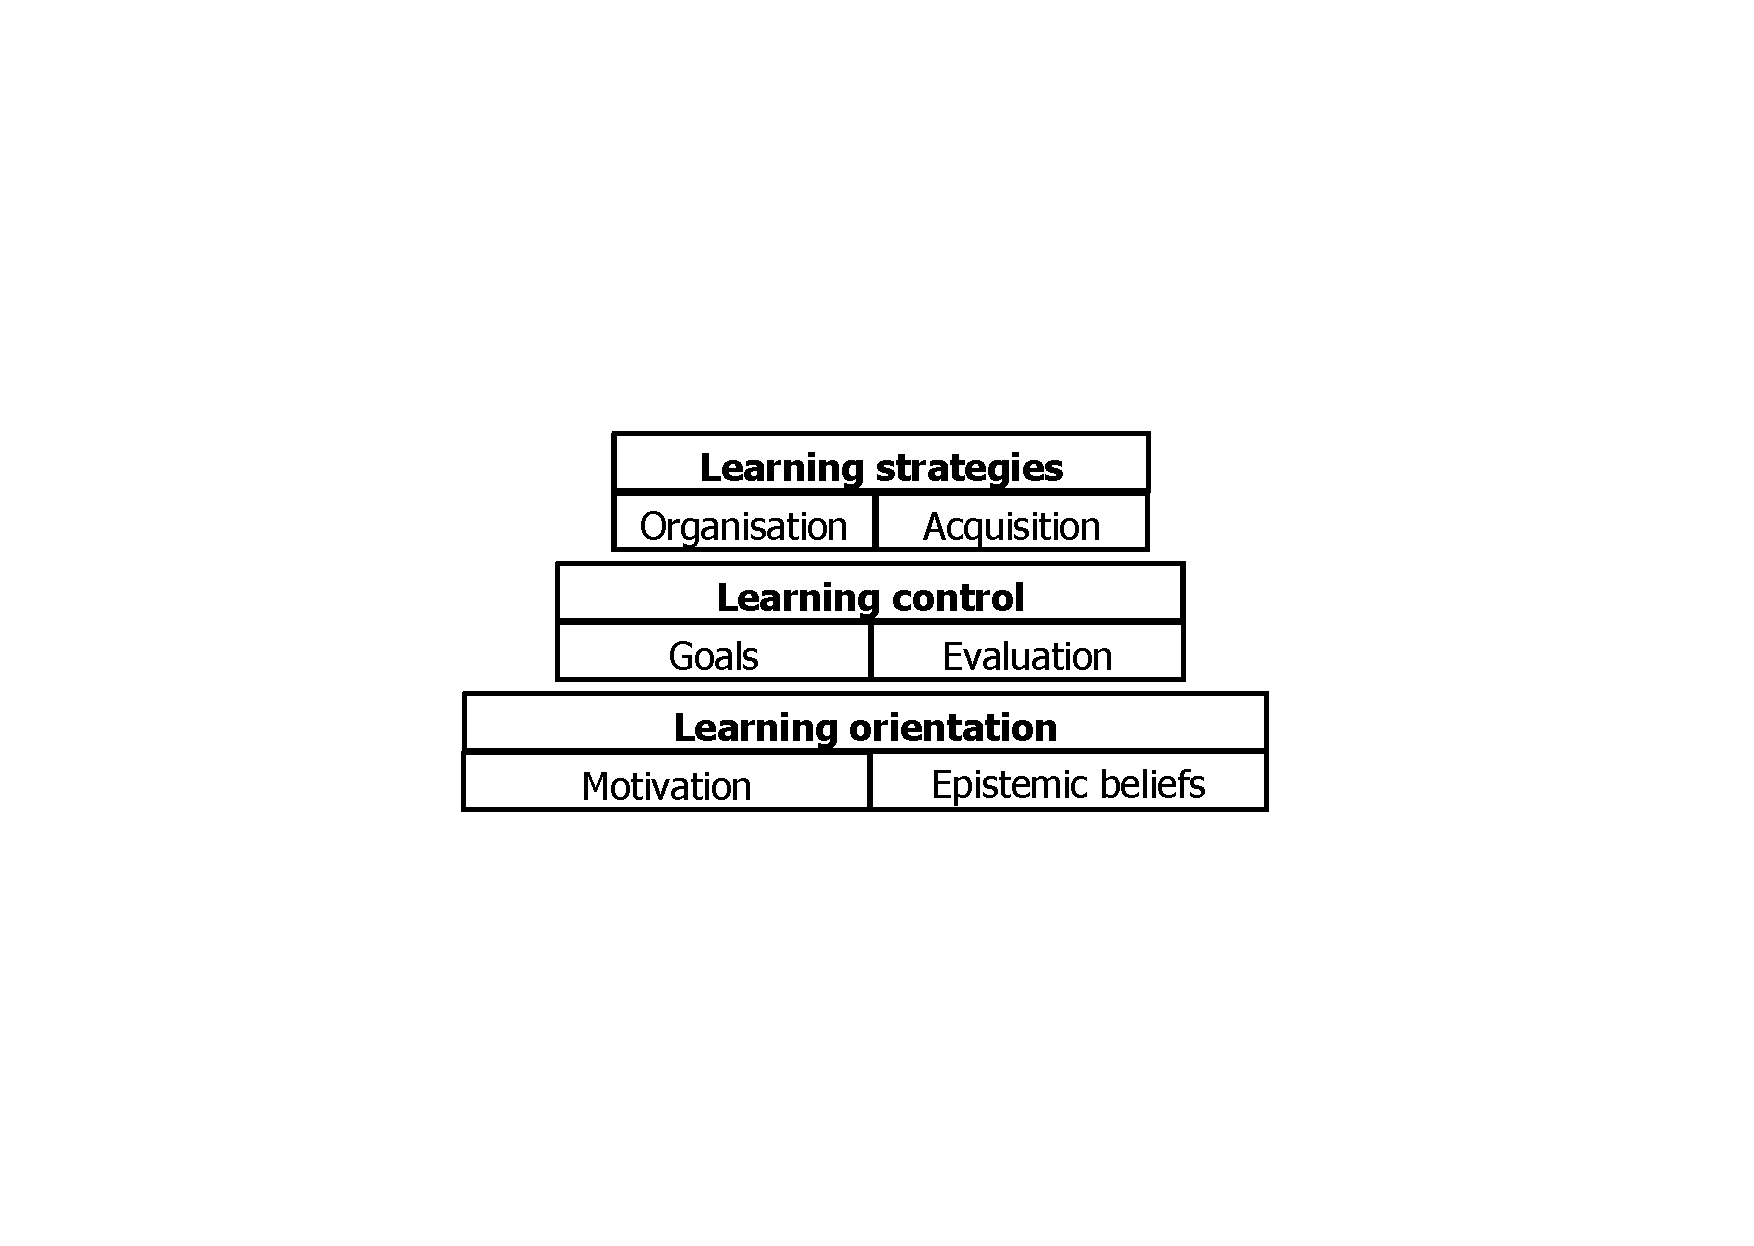
\includegraphics[width=0.5\textwidth,height=8cm]{RR2008CSRImage.pdf}
    \caption{Levels and central constructs of learning competency.}
  \end{center}
\end{figure}

\begin{flushleft}
\textbf{Research Highlights 2007/2008}
\end{flushleft}

We began with employee surveys assessing the interplay of meta-cognitive and motivational variables, and the influence of organizational variables (e.g., T\&D climate, learning opportunities at work) on learning competency. Results indicated that older workers showed learning competency decreases from declines in memory self-efficacy (MSE) rather than as a function of biological age. As such declines are particularly likely in organizations that offer few learning opportunities, and that fail to encourage continuous T\&D participation, older workers are more likely than their younger colleagues to experience MSE decline; it may thus be seen as a secondary age effect. We follow up on these findings in laboratory research investigating the interplay of age, MSE, and task difficulty in cognitive resource allocation to self-regulated learning tasks in an e-learning environment. Intervention studies follow naturally from this approach, and thus they form a third focus of our research. We have started designing "learning competency workshops" that seek to enhance learning performance by training goal-setting and monitoring skills.


\subsubsection{Age-Related Changes in Work Motivation }


\begin{flushleft}
\textbf{Research Program}
\end{flushleft}


Given decreasing numbers of young workforce entrants, the successful retention of older workers is of high importance for many organizations; this requires a profound understanding of older workers' motivation. While aging, more often than not, is perceived to involve inevitable decline in motivation, we posit that age-related changes in work motivation might be conceptualized as outcomes of active regulation. Rather than passively responding to personal (e.g., capability declines) and environmental (e.g., altered work demands) changes, older workers actively adapt to these changes. As a result, work motivation becomes more task-specific; the influence of work context on motivation changes both quantitatively and qualitatively and leads to developing an individual motivational profile (Stamov Ro�nagel, in press).

\paragraph{}
In co-operation with various companies, we develop within this framework tools for motivation diagnostics and interventions. We seek to identify specific areas of age-related increases and decreases. Beyond academic interest, conceptualizing age-related changes in motivation as an outcome of active regulation might provide human resource professionals with more opportunities for motivation interventions. For instance, giving older workers higher degrees of job control might help fulfill their needs for job customization, and may enable them to allocate effort in line with their motivational profile. In a similar vein, discussing and "teaching" motivational regulation strategies might help equip older workers with skills to successfully cope with age-related capability changes and changing job demands. Finally, research into motivation profiles might increase the effectiveness and efficiency of motivational interventions, and might be fruitful for building (age-diverse) teams.

\paragraph{}
\begin{flushleft}
\textbf{Research Highlights 2007/2008}
\end{flushleft}

In a recently completed survey, we asked 312 workers (ages 18-65) from a company to rate how motivated they were for their work in general and for tasks emphasizing collaboration with colleagues, demonstration of one's knowledge and skills, learning new skills or knowledge, leading others, working autonomously, and passing to colleagues one's knowledge and experience, respectively. Moreover, to assess needs-supplies fit, participants indicated whether they felt they were given sufficient opportunities to work on each of these task types. We found that the motivation patterns as defined by the six aforementioned types of tasks differed as a function of age. Most importantly, older workers showed higher levels of motivation than their younger colleagues on the "people tasks" involving passing on knowledge and experience and leading others. Independent of age, the overall level of motivation was higher for participants who reported good fit, that is, older workers who reported high needs-supplies fit rated their overall motivation on a comparable level than their younger colleagues. Also, high levels of fit were associated with positive affect at work, indicating that task-specific motivation regulation might be a useful strategy of affect regulation.


\subsubsection{Older Workers' Cognitive Resources for Innovation Behavior }



Most recently, we have embarked on innovation behavior research, which will be funded by a Volkswagen Foundation grant until 2011. Similar to the situation with workplace learning and motivation research, older workers have been somewhat neglected in this field. Although the demand for innovation increases in the wake of technological change and globalization, and although a growing number of older workers will be involved in innovation-related work roles, little research has dealt with the question how age might affect innovation behavior.

\paragraph{} 
Our research focuses on the motivation-cognition interface. We assume that while aging might objectively affect older workers' cognitive innovation resources, workers will strive to compensate for declining resources availability if such compensation is supported by the organization. Routinization, a facet of expertise, is a resource of particular interest in this regard. It frees up cognitive capacity that in an innovation-supporting environment might be directed towards recognizing innovation potentials and developing implementation strategies. In a less supportive environment, however, routinization may be married with unproductive routine. Like for our workplace learning and motivation research, we develop a combination of quantitative survey and experimental methods to investigate the role of personal cognitive resources.


\subsubsection{Collaborators }

%\input{326}
\begin{itemize}
\item University of Heidelberg; \\Sonja Bausch.
\item University of Dortmund;\\ Michael Falkenstein.
\item University of Oldenburg;\\ Prof. Dr. Barbara Moschner.
\item University of Passau;\\ Prof. Dr. Franz Lehner.
\item Portland State University;\\ Prof. Dr. Pamela Tierney.
\item Bremen-Nord Hospital.
\item Deutsche Bank.
\item EnBW.
\item HeidelbergCement.
\item OTTO Group.
\end{itemize}


\subsubsection{Other Professional Activities }


\textit{Ad-hoc reviews:}
Applied Psychology: An International Review, European Journal of Personality, Journal of Behavioural Sciences, Zeitschrift f�r Personalpsychologie, Zeitschrift f�r Sozialpsychologie. \\

\textit{Boards 2007/2008}

\begin{itemize}
\item EU Commission. Member of the Board of Judges, \textit{European Union eInclusion Awards.}
\item Federal Institute of Occupational Health and Safety (BAuA), Advisory Board Member of the PFIFF project.
\end{itemize}

\subsubsection{Publications }

\begin{itemize}

\item Stamov Ro�nagel, C. (in press). Motivationsregulation �lterer Besch�ftigter. In K. Brauer \& G. Korge, editor, \textit{Perspektive 50plus? Theoretische und Praktische Ans�tze zur regionalen Arbeitsmarktf�rderung �lterer.} Wiesbaden: Verlag f�r Sozialwissenschaften. 

\item Stamov Ro�nagel, C. (in press). Arbeitsmotivation �ber die Lebensspanne: Aktive Regulation statt passiven Abbaus. In J. Kocka, M. Kohli, \& W. Streeck (Hrsg.), \textit{Altern, Familie, Zivilgesellschaft und Politik.} Stuttgart: Wissenschaftliche Verlagsgesellschaft.

\item Stamov Ro�nagel, C. (in press). Was H�nschen nicht lernt...? Folgen der Altersselektion bei Weiterbildungskonzepten. In K. Brauer \& W. Clemens (Hrsg.).\textit{ Zu Alt? Zur Theorie des Ageism und zur Empirie der Altersdiskriminierung auf Arbeitsm�rkten}. Wiesbaden: Verlag f�r Sozialwissenschaften.

\item Gotoh, F., Kikuchi, T., \& Stamov Ro�nagel, C. (2008). Emotional Interference in Enumeration: A Working Memory Perspective. \textit{Psychology Science Quarterly}, 50 (4), 526-537.

\item Stamov Ro�nagel, C. (2008). Motivationsregulation �lterer Besch�ftigter. In K. Brauer \& G. Korge (Eds.), \textit{Perspektive 50plus? Theoretische und Praktische Ans�tze zur regionalen Arbeitsmarktf�rderung �lterer} (p. 71-86). Wiesbaden: Verlag f�r Sozialwissenschaften.

\item Stamov Ro�nagel, C. (2008). \textit{Mythos "Alter Mitarbeiter": Lernkompetenz jenseits der 40}? Weinheim: Beltz PVU.

\item Stamov Ro�nagel, C., Picard, M.A., \& Voelpel, S. (2008). Weiterbildung jenseits der 40. \textit{Personal}, 36-38.

\item Lehner, F. \& Ro�nagel, C. (2008). iVideo - An Easy-to-use Authoring Tool for Interactive E-Learning Videos. In Luca, J. \& Weippl, E.R. editors, \textit{Proceedings of ED-MEDIA 2008 - World Conference on Educational Multimedia, Hypermedia \& Telecommunications} (5373 - 5378). Chesapeake, VA: AACE. 

\item Staudinger, U. M., Ro�nagel, C., \& V�lpel, S. (2008). Strategische Personalentwicklung und demographischer Wandel - eine interdisziplin�re Perspektive. In K. Schwuchow \& J. Gutmann, J., editors, \textit{Jahrbuch Personalentwicklung 2008 - Ausbildung, Weiterbildung, Management Development} (295-304). M�nchen: Luchterhand.

\item Ro�nagel, C. \& Schulz, M. (2007). Besch�ftigungsf�higkeit erfahrener Mitarbeiter. sichern - welche Rolle spielt die betriebliche Weiterbildung Ergebnisse einer Befragung von Unternehmen in Ostwestfalen-Lippe. G�tersloh: Bertelsmann.

\item Ro�nagel, C. \& Voelpel, S. (2007). Qualifizierung �lterer Mitarbeiter: Keine Einheitsweiterbildung. \textit{Persorama}, 35, 24-29.

\end{itemize}